%\PassOptionsToPackage{english}{babel}
% \RequirePackage{fix-cm}
\documentclass[final,t]{beamer}
\usefonttheme{professionalfonts}
\mode<presentation>
{
%  \usetheme{Warsaw}
%  \usetheme{Aachen}
%  \usetheme{Oldi6}
%  \usetheme{I6td}
  \usetheme{I6dv}
%  \usetheme{I6pd}
%  \usetheme{I6pd2}
}
% additional settings
\setbeamerfont{itemize}{size=\normalsize}
\setbeamerfont{itemize/enumerate body}{size=\normalsize}
\setbeamerfont{itemize/enumerate subbody}{size=\normalsize}

\usepackage{xfrac}
\usepackage{mathrsfs}

\DeclareFontFamily{U}{rsfs}{\skewchar\font127 }
\DeclareFontShape{U}{rsfs}{m}{n}{%
   <-6> rsfs5
   <6-8> rsfs7
   <8-> rsfs10
}{}

\usepackage{algorithm}
% \usepackage{algorithmic}
\usepackage[noend]{algpseudocode}


\usepackage{Definitions}
\usepackage{tensor}
\usepackage{empheq}
\usepackage{array}
% \usepackage{color}
% \usepackage[usenames,dvipsnames,svgnames,table]{xcolor}
% \usepackage{tikz}
% \usetikzlibrary{calc}

% additional packages
\usepackage{times}
\usepackage{amsmath,amsthm, amssymb, latexsym}
\usepackage{exscale}

\usepackage{graphicx} % more modern
\usepackage{wrapfig}
% \usepackage{subfigure}
% \usepackage{caption}

% \boldmath
\usepackage{booktabs, array}
% \usepackage{rotating} %sideways environment
\usepackage[english]{babel}
\usepackage[latin1]{inputenc}
\usepackage[orientation=landscape,size=custom,width=155,height=90,scale=1.4]{beamerposter}
\listfiles
\graphicspath{{figure/}}
\usepackage{ragged2e}

\newenvironment<>{thmblock}[2][1\textwidth]{%
  \setlength{\textwidth}{#1}
\setbeamertemplate{blocks}[rounded][shadow=true]
  \begin{actionenv}#3%
    \def\insertblocktitle{#2}%
    \par%
    \usebeamertemplate{block begin}}
  {\par%
    \usebeamertemplate{block end}%
  \end{actionenv}}

\newcommand{\algabb}{BASE}

\title{Nonparametric Teaching for Multiple Learners\\}

\author{ \Large
  Chen Zhang$^1$, Xiaofeng Cao$^1$, Weiyang Liu$^{2,3}$, Ivor W. Tsang$^{4}$, James T. Kwok$^{5}$
}

% abbreviations
\usepackage{xspace}
\makeatletter
\DeclareRobustCommand\onedot{\futurelet\@let@token\@onedot}
\def\@onedot{\ifx\@let@token.\else.\null\fi\xspace}
\makeatother

\begin{document}
\begin{frame}
\vspace{-0.4in}
\begin{columns}[t]

%======================First coloumn
\begin{column}{.27\linewidth}
%-----------------block 1---------------
\begin{block}{Machine Teaching}
Machine teaching (MT) considers the problem of how to design \alert{the most effective teaching set}, typically with the \alert{smallest amount} of (teaching) examples possible, to facilitate rapid learning of the \alert{target models} by learners based on these examples. 

\vspace{6mm}

It can be thought of as an \alert{inverse} of machine learning, in the sense that the learner is to learn models on a given dataset, while the teacher is to seek a (minimal) dataset from a target model.

\vspace{6mm}

Depending on how teachers and learners \alert{interact} with each other, MT can be carried out in either\begin{itemize}
\justifying
    \item {\color{blue} batch} fashion which focuses on \alert{single-round} interaction, that is, the most representative and effective teaching dataset are designed to be fed to the learner in one shot, or 
    \item {\color{blue} iterative} fashion where an iterative teacher would feed  examples based on learners' status (current learnt models) \alert{round by round}, such that the learner can converge to a target model within fewer rounds.
\end{itemize}
\end{block}

%-----------------block 2---------------
\begin{block}{Motivation}

\begin{wrapfigure}{R}{0.4\textwidth}
  \centering
  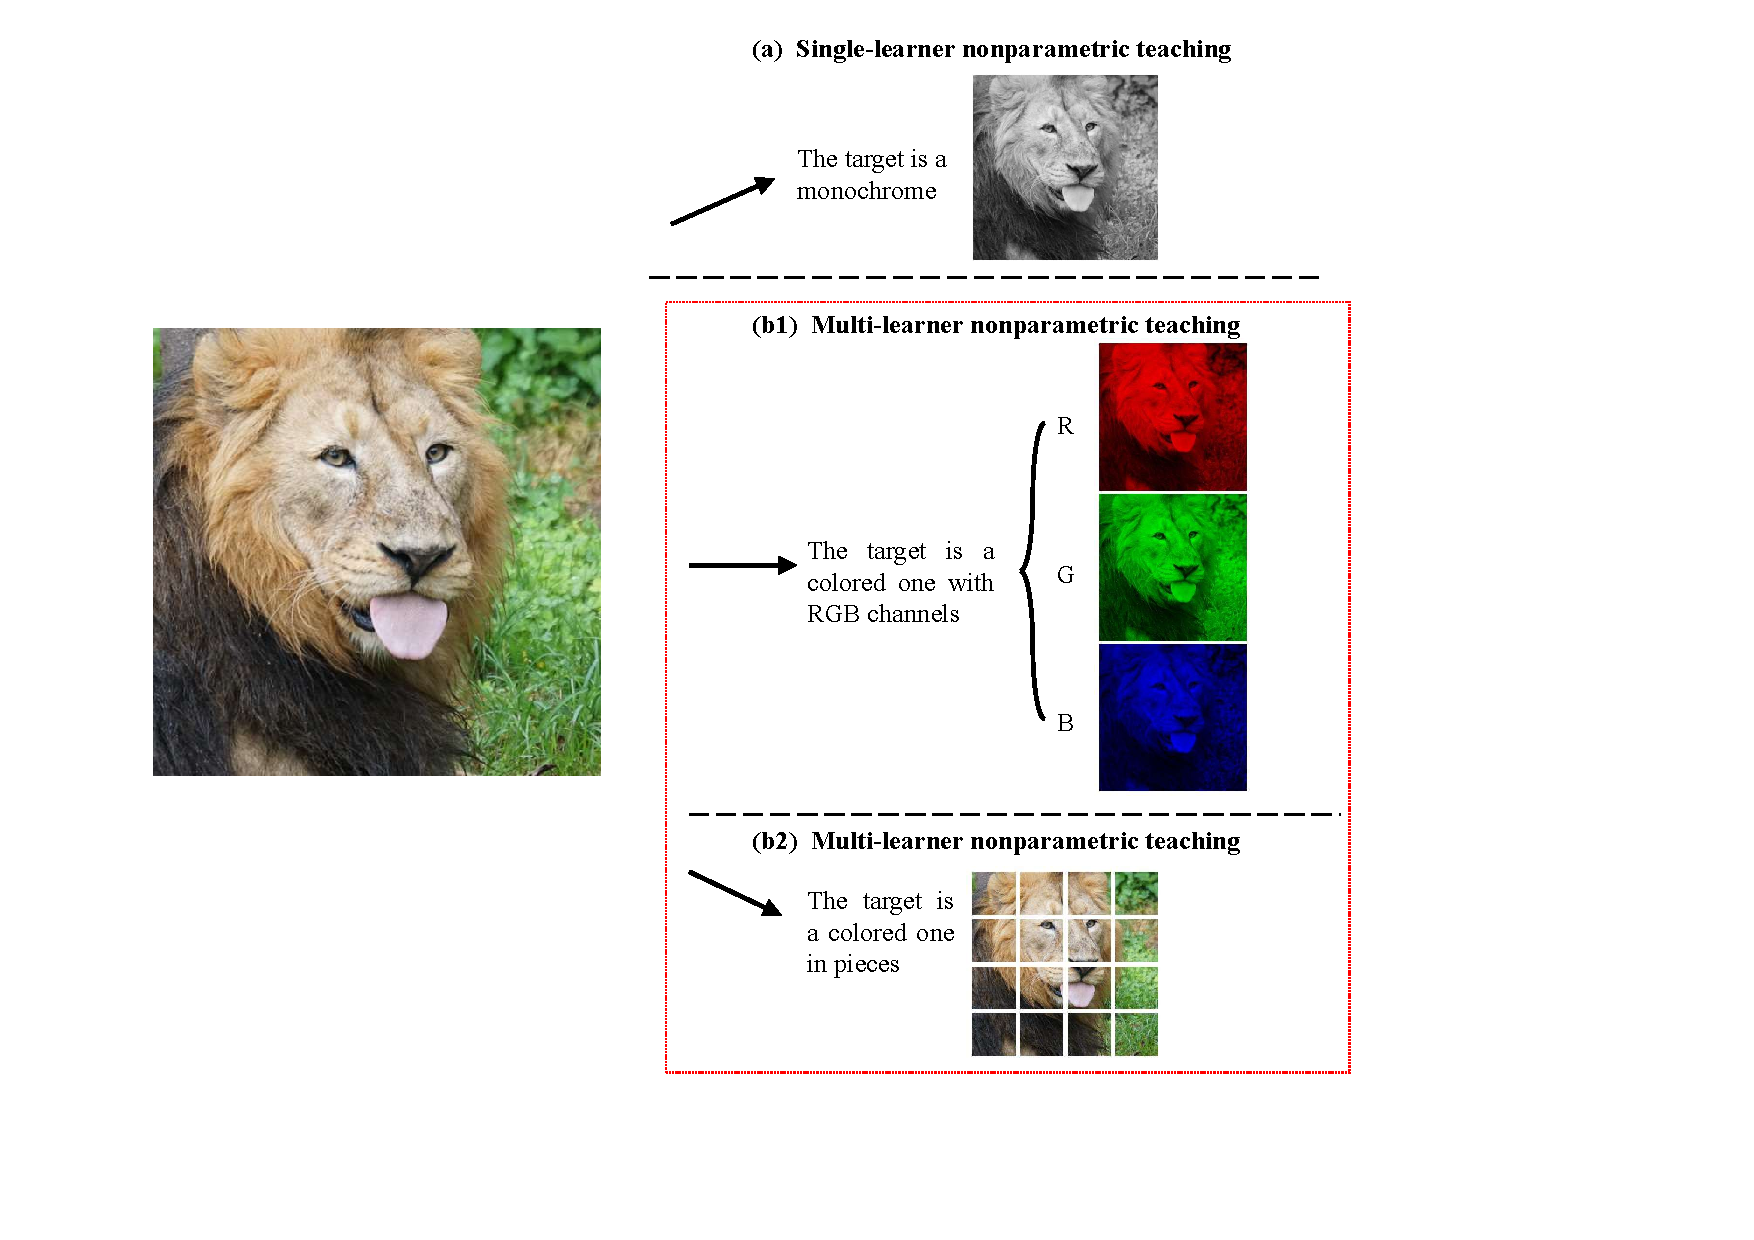
\includegraphics[width=0.35\textwidth]{comp.pdf}
  \caption{\footnotesize Comparison between the single-learner teaching and MINT.}
  \label{fig}
\end{wrapfigure}


Previous nonparametric teaching algorithms merely focus on the \alert{single-learner setting} (\ie, teaching a \alert{scalar-valued} target model or function to a single learner). To empower them to fulfill the practical needs of complex tasks, we introduce a more comprehensive task called {\bf Multi-learner Nonparametric Teaching} (MINT). In MINT, the teacher aims to instruct \alert{multiple learners}, with each learner focusing on learning a \alert{scalar-valued} target model.


\vspace{4mm}
      {\bf \color{blue} Main Contribution}: 
\begin{itemize}
\justifying
\item By analyzing general \alert{vector-valued RKHS}, we study the {\bf multi-learner nonparametric teaching} (MINT), where the teacher selects examples based on a \alert{vector-valued target function} (each component of it is a scalar-valued one for a single learner) such that \alert{multiple} learners can learn its components simultaneously in a fast speed. 
\item By enabling the \alert{communication} among multiple learners, learners can update themselves with a \alert{linear combination} of current learnt functions of all learners. We study a communicated MINT where the teacher not only selects examples but also injects the \alert{guidance} of communication.
\item Under mild assumptions, we characterize the \alert{efficiency} of our \alert{multi-learner generalization} of nonparametric teaching. More importantly, we also \alert{empirically} demonstrate its efficiency.
\end{itemize}
\vspace{-7mm}
\end{block}
\end{column}


%======================Second coloumn
\begin{column}{.37\linewidth}
%-----------------block 1---------------
\begin{block}{Teaching Settings}
{\bf \color{blue} Vector-valued Functional Optimization}: We define multi-learner noparametric teaching as a \alert{vector-valued functional minimization} over the collection of potential teaching sequences $\mathbb{D}$ in the vector-valued reproducing kernel Hilbert space:
\begin{equation}\label{eq1}
\bm{\mathcal{D}}^*=\underset{\bm{\mathcal{D}}\in\mathbb{D}^d}{\arg\min}\quad \mathcal{M}(\hat{\bm{f}^*},\bm{f}^*)+\lambda\cdot \text{len}(\bm{\mathcal{D}}) \qquad \text{s.t.}\quad\hat{\bm{f}^*}=\mathcal{A}(\bm{\mathcal{D}})
\end{equation}
where $\mathcal{M}$ denotes a discrepancy measure, $\text{len}(\bm{\mathcal{D}})$, 
which is regularized by a constant $\lambda$, is the length of the teaching sequence $\bm{\mathcal{D}}$, and $\mathcal{A}$ represents the learning algorithm of learners. Specifically, $\mathcal{A}$ is taken as $\hat{\bm{f}^*}=\underset {\bm{f}\in\mathcal{H}^d}{\arg\min}\,\mathbb{E}_{(\bm{x},\bm{y})}\left[\mathcal{L}(\bm{f}(\bm{x}),\bm{y})\right]$,
where $(\bm{x},\bm{y})\in\mathcal{X}^d\times\mathcal{Y}^d$ and $(\bm{x},\bm{y})\sim[\mathbb{Q}_i(x_i,y_i)]^d$. Evaluated at an example vector $(\bm{x},\bm{y})=[(x_{i,j_i},y_{i,j_i})]^d$ with the example index $j_i\in\mathbb{N}_k$, the \alert{multi-learner convex} loss $\mathcal{L}$ therein is
$\mathcal{L}(\bm{f}(\bm{x}),\bm{y})=\sum_{i=1}^d \mathcal{L}_i(f_i(x_{i,j_i}),y_{i,j_i})=E_{\bm{x}}\left[[\mathcal{L}_i(f_i,y_{i,j_i})]^d\right]$, where $\mathcal{L}_i$ is the \alert{convex} loss for $i$-th learner.


\end{block}

%-----------------block 2---------------
\begin{block}{Vanilla Multi-learner Teaching}
\textbf{Lemma 1} (Sufficient Descent for multi-learner \textbf{RFT}). Suppose there are $d$ learners, and the example \alert{mean} for each learner is $\mu_i=\mathbb{E}_{x_i\sim\mathbb{P}_i(x_i)}(x_i)<\infty$, and the \alert{variance} $\sigma_i^2=\mathbb{E}_{x_i\sim\mathbb{P}_i(x_i)}(x_i-\mu_i)^2<\infty, i\in\mathbb{N}_d$. Under the \alert{Lipschitz smooth and bounded kernel assumptions}, if $\eta^t_i\leq \frac{1}{2L_\mathcal{L}\cdot M_K}$ for all $i\in\mathbb{N}_d$, then RFT teachers can, \alert{on average}, reduce the multi-learner loss $\mathcal{L}(\bm{f})$ by:
\begin{eqnarray}
\mathbb{E}_{\bm{x}\sim[\mathbb{P}_i(x_i)]^d}\left[\mathcal{L}(\bm{f}^{t+1})-\mathcal{L}(\bm{f}^t)\right]\leq-\frac{\tilde{\eta}^t}{2}\sum_{i=1}^d (m_{i,t}(\mu_i)+\frac{m_{i,t}''(\mu_i)}{2}\sigma_i^2),
\end{eqnarray}
	where $\tilde{\eta}^t=\min_{i\in\mathbb{N}_d}\eta^t_i$ and $m_{i,t}(\dot{x})\coloneqq E_{\dot{x}}[(\left.\nabla_f\mathcal{L}_i(f)\right|_{f=f^{t}_i})^2]$.

\vspace{6mm}

\textbf{Theorem 2} (Convergence for multi-learner \textbf{RFT}). Suppose the \alert{vector-valued} model for multiple learners is initialized with $\bm{f}^0\in\mathcal{H}^d$ and returns $\bm{f}^t\in\mathcal{H}^d$ after $t$ iterations, we have the \alert{upper bound} of $\min_{i\in\mathbb{N}_d} \left(m_{i,t}(\mu_i)+m_{i,t}''(\mu_i)\sigma_i^2/2\right)$ w.r.t. $t$:
	\begin{eqnarray}\label{eqcpft}
		\min_{i\in\mathbb{N}_d} \left(m_{i,t-1}(\mu_i)+m_{i,t-1}''(\mu_i)\sigma_i^2/2\right)\leq2\mathbb{E}_{\bm{x}\sim[\mathbb{P}_i(x_i)]^d}\left[\mathcal{L}(\bm{f}^0)\right]/(d\dot{\eta}t),
	\end{eqnarray}
	where $0<\dot{\eta}=\underset{l\in\{0\}\bigcup\mathbb{N}_{t-1}}{\min}\,\tilde{\eta}^l\leq 1/(2L_\mathcal{L}\cdot M_K)$, and given a small constant $\epsilon>0$ it would take approximately $\mathcal{O}(2\mathbb{E}_{\bm{x}\sim[\mathbb{P}_i(x_i)]^d}\left[\mathcal{L}\left(\bm{f}^0)\right]/(d\dot{\eta}\epsilon)\right)$ iterations to reach a \alert{stationary point}.

\vspace{6mm}

\textbf{Lemma 3} (Sufficient Descent for multi-learner \textbf{GFT}). Under the same assumption, if $\eta^t_i\leq \frac{1}{2L_\mathcal{L}\cdot M_K}$ for all $i\in\mathbb{N}_d$, the GFT teachers can achieve a \alert{greater} reduction in the multi-learner loss $\mathcal{L}$:
	\begin{eqnarray}
		\mathbb{E}_{\bm{x}\sim[\mathbb{P}_i(x_i)]^d}\left[\mathcal{L}(\bm{f}^{t+1})-\mathcal{L}(\bm{f}^t)\right]\leq-\frac{\tilde{\eta}^t}{2}\sum_{i=1}^d m_{i,t}({x^t_i}^*),
	\end{eqnarray}
	where $\tilde{\eta}^t$ and $m_{i,t}(\cdot)$ retain their previous meaning.

\vspace{6mm}

\textbf{Theorem 4} (Convergence for multi-learner \textbf{GFT}). Suppose the \alert{vector-valued} model for multiple learners is initialized with $\bm{f}^0\in\mathcal{H}^d$ and returns $\bm{f}^t\in\mathcal{H}^d$ after $t$ iterations, we have the \alert{upper bound} of $\min_{i\in\mathbb{N}_d} m_{i,t}({x^t_i}^*)$ w.r.t. $t$:
	\begin{eqnarray}\label{eqcgft}
		\min_{i\in\mathbb{N}_d} m_{i,t-1}({x^{t-1}_i}^*)\leq\frac{2}{d\dot{\eta}t}\mathbb{E}_{\bm{x}\sim[\mathbb{P}_i(x_i)]^d}\left[\mathcal{L}(\bm{f}^0)\right]+\frac{1}{d}\sum_{l=0}^{t-1}\sum_{i=1}^d \left(\|{x^l_i}^*-\mu_i\|_2\right),
	\end{eqnarray}
	where $\dot{\eta}$ has the same definition as before.

\end{block}
      
\end{column}


%======================Third coloumn
\begin{column}{0.28\linewidth}
%-----------------block 3---------------
\begin{block}{Communicated Multi-learner Teaching}
\textbf{Proposition 5} If the proximity between $\bm{f}^t$ and $\bm{f}^*$ is \alert{sufficiently close}, meaning that $\|\bm{f}^t-\bm{f}^*\|_{\mathcal{H}^d}\leq\epsilon$ where $\epsilon$ is a tiny positive constant, then $A^t$ equals the \alert{identity matrix} $I_d$.

\textbf{Lemma 6}
Under \alert{Lipschitz smooth} assumption, the \alert{communication} across learners will result in a \alert{reduction} of the \alert{multi-learner convex} loss $\mathcal{L}$ by  $0\leq\mathcal{L}(\bm{f}^t)-\mathcal{L}(A^t\bm{f}^t)\leq2L_\mathcal{L}\|\bm{f}^t-\bm{f}^*\|_{\mathcal{H}^d}$.

\textbf{Theorem 7} Suppose the \alert{communication} in the $t$-th iteration of multiple learners is denoted by the \alert{matrix} $A^t$ and returns $\bm{f}^{t+1}_{A^t}\in\mathcal{H}^d$, for both RFT and GFT we have:
	$$\mathbb{E}_{\bm{x}\sim[\mathbb{P}_i(x_i)]^d}\left[\mathcal{L}(\bm{f}^{t+1}_{A^t})-\mathcal{L}(\bm{f}^t)\right]\leq
		\mathbb{E}_{\bm{x}\sim[\mathbb{P}_i(x_i)]^d}\left[\mathcal{L}(\bm{f}^{t+1}_{A^t})-\mathcal{L}(A^t\bm{f}^t)\right]\leq0.$$
 
\end{block}

\begin{block}{Experiments and Results}

\begin{itemize}
    \item {\bf MINT in gray scale.}
\end{itemize}

\centering
\vspace{6mm}
\begin{tabular}{lclc}
{\color{blue} Simultaneous teaching of a tiger and a cheetah.} \vspace{-8mm}\\

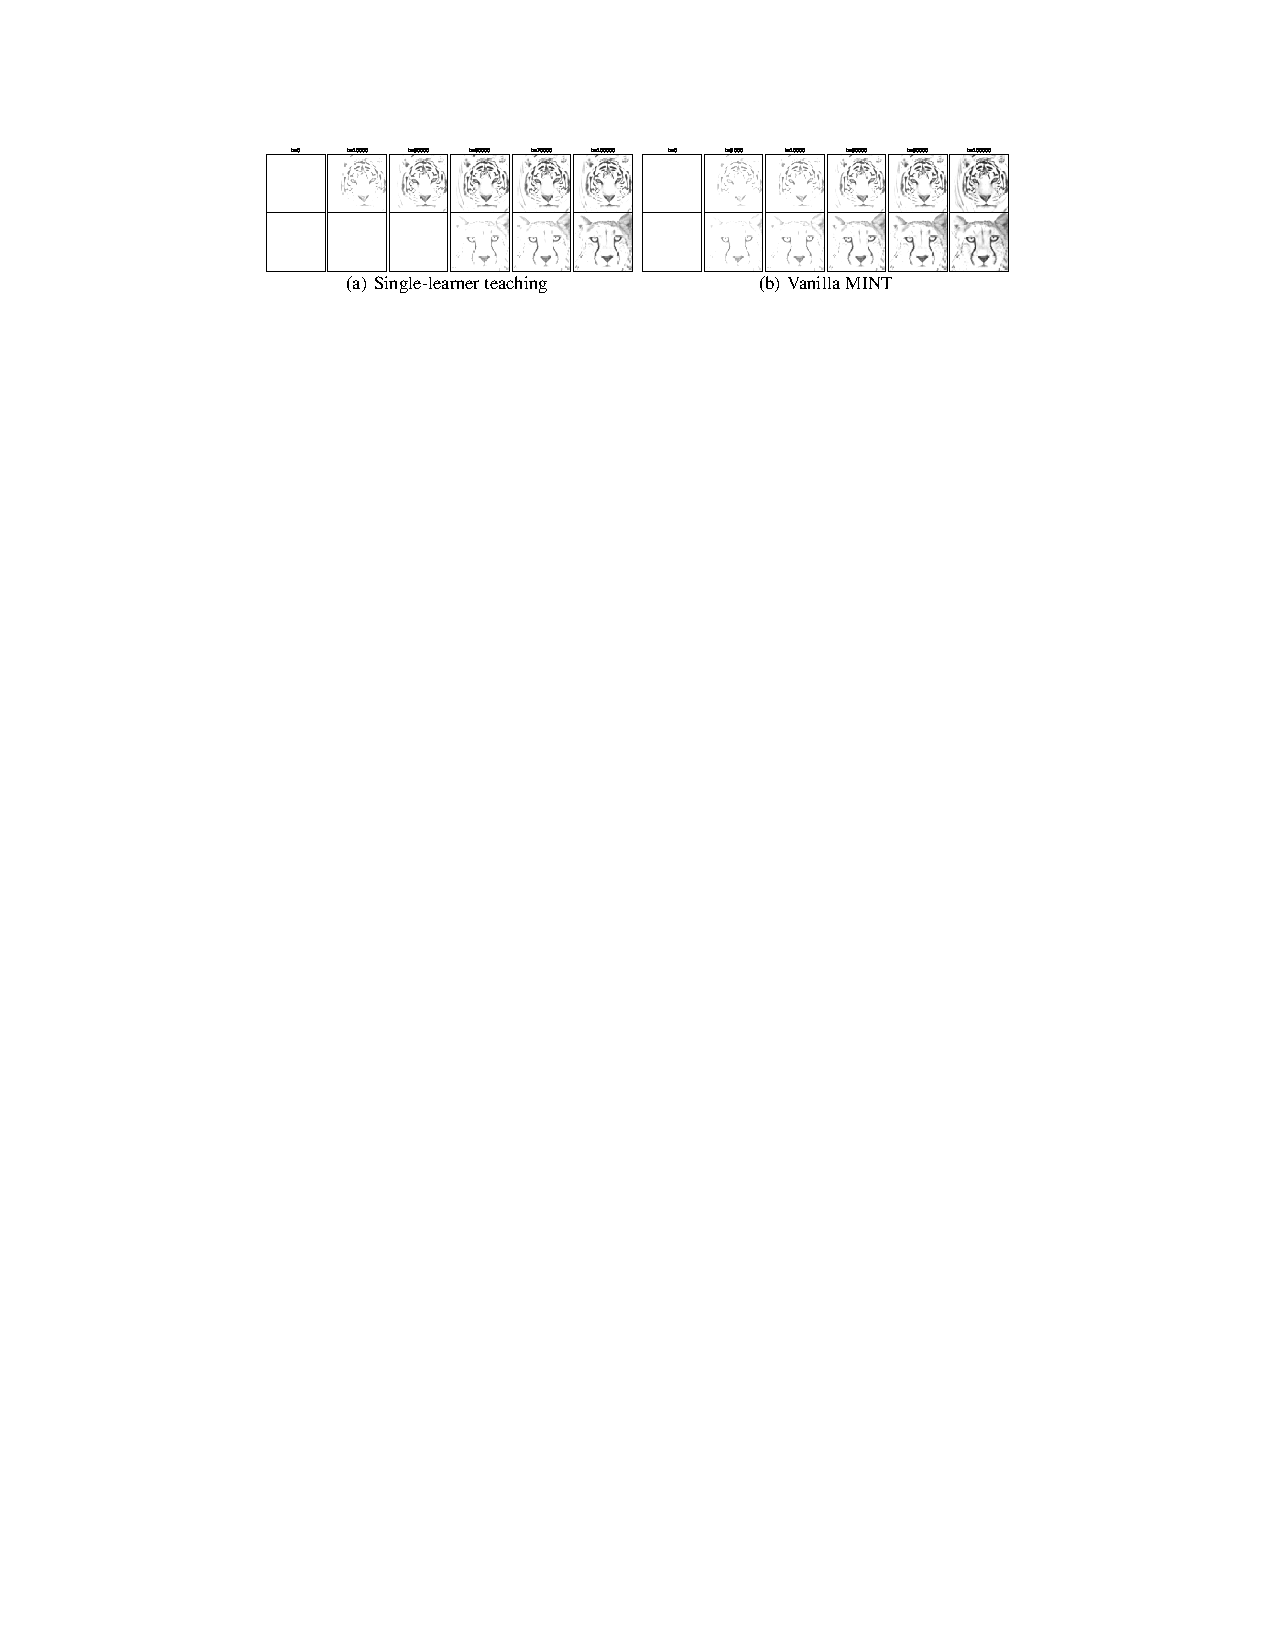
\includegraphics[width=\linewidth]{./out/grayTigerCheetah}\\
{\color{blue} Teaching of a lion by partition.}\vspace{-3mm}\\

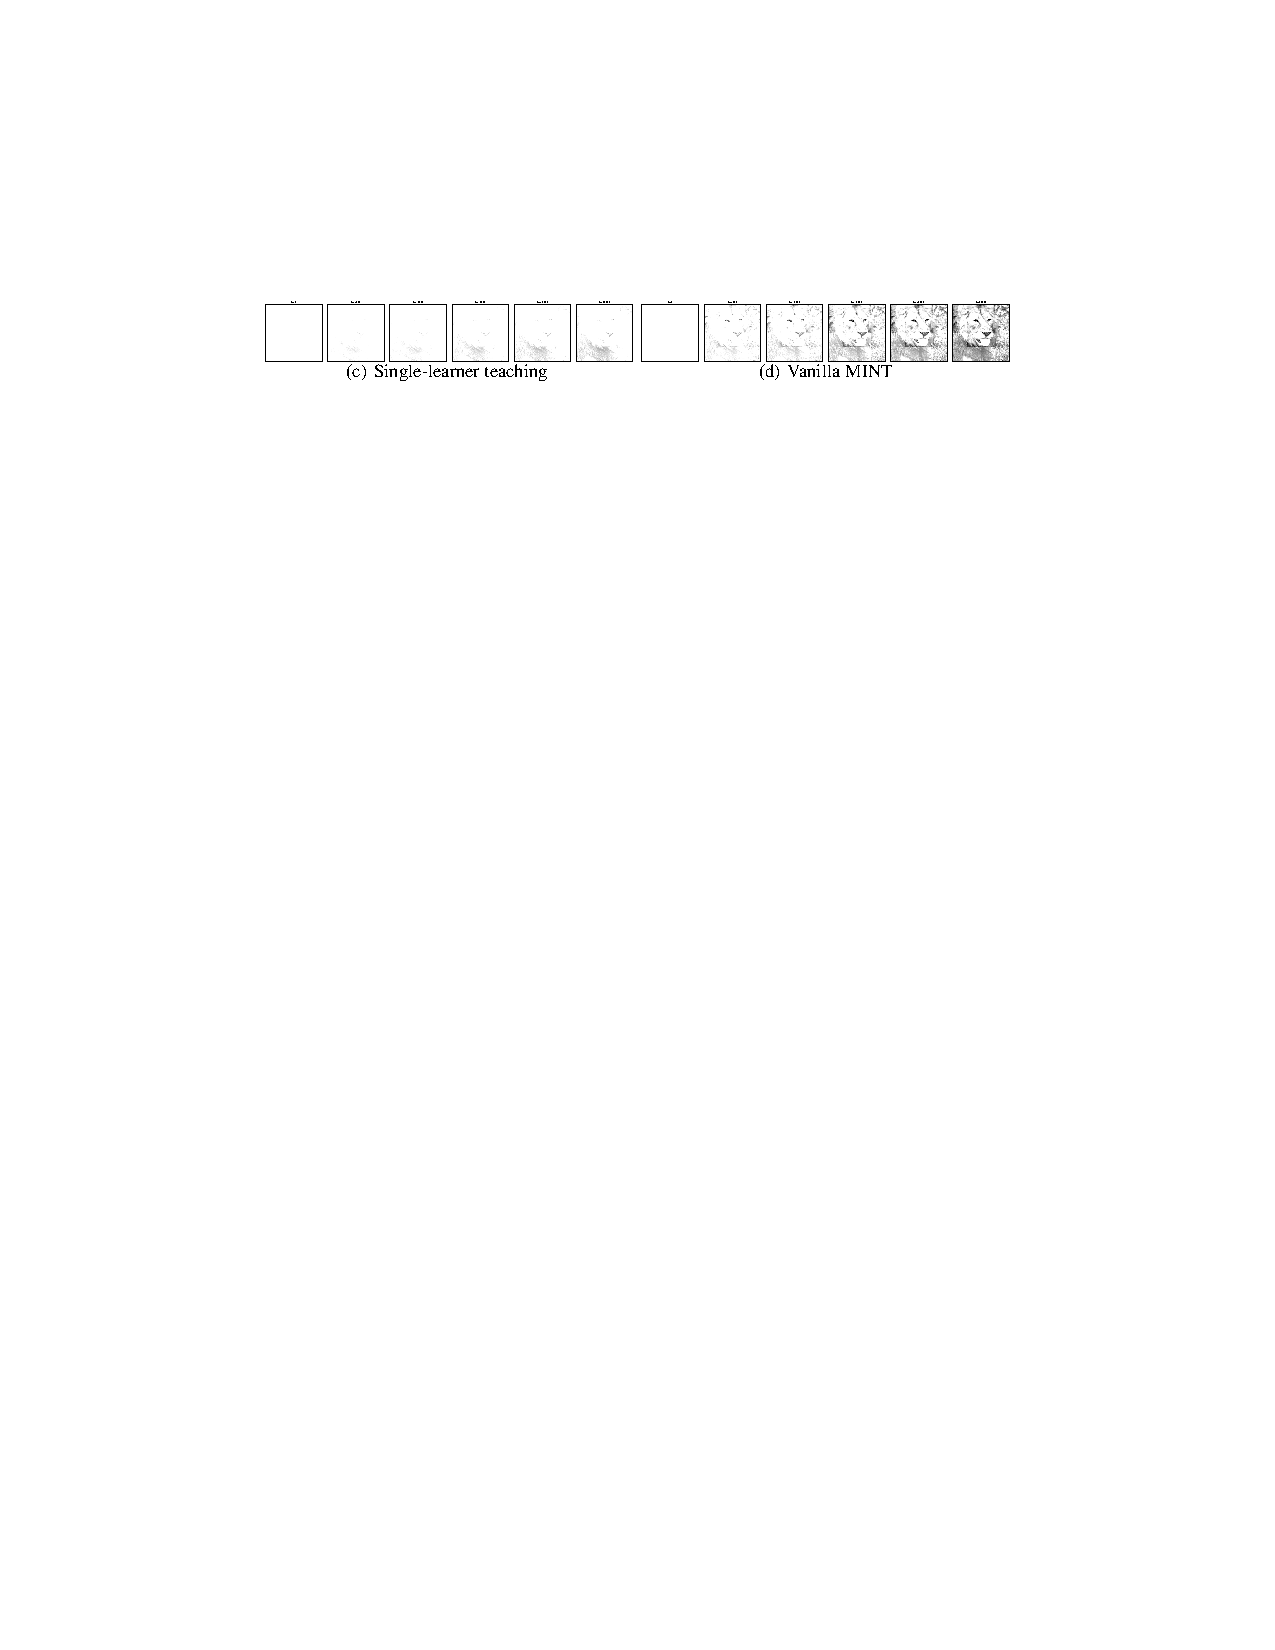
\includegraphics[width=\linewidth]{./out/grayLion}\\
\end{tabular}

\vspace{6mm}

\begin{itemize}
    \item {\bf  MINT in three (RGB) channels.}
\end{itemize}


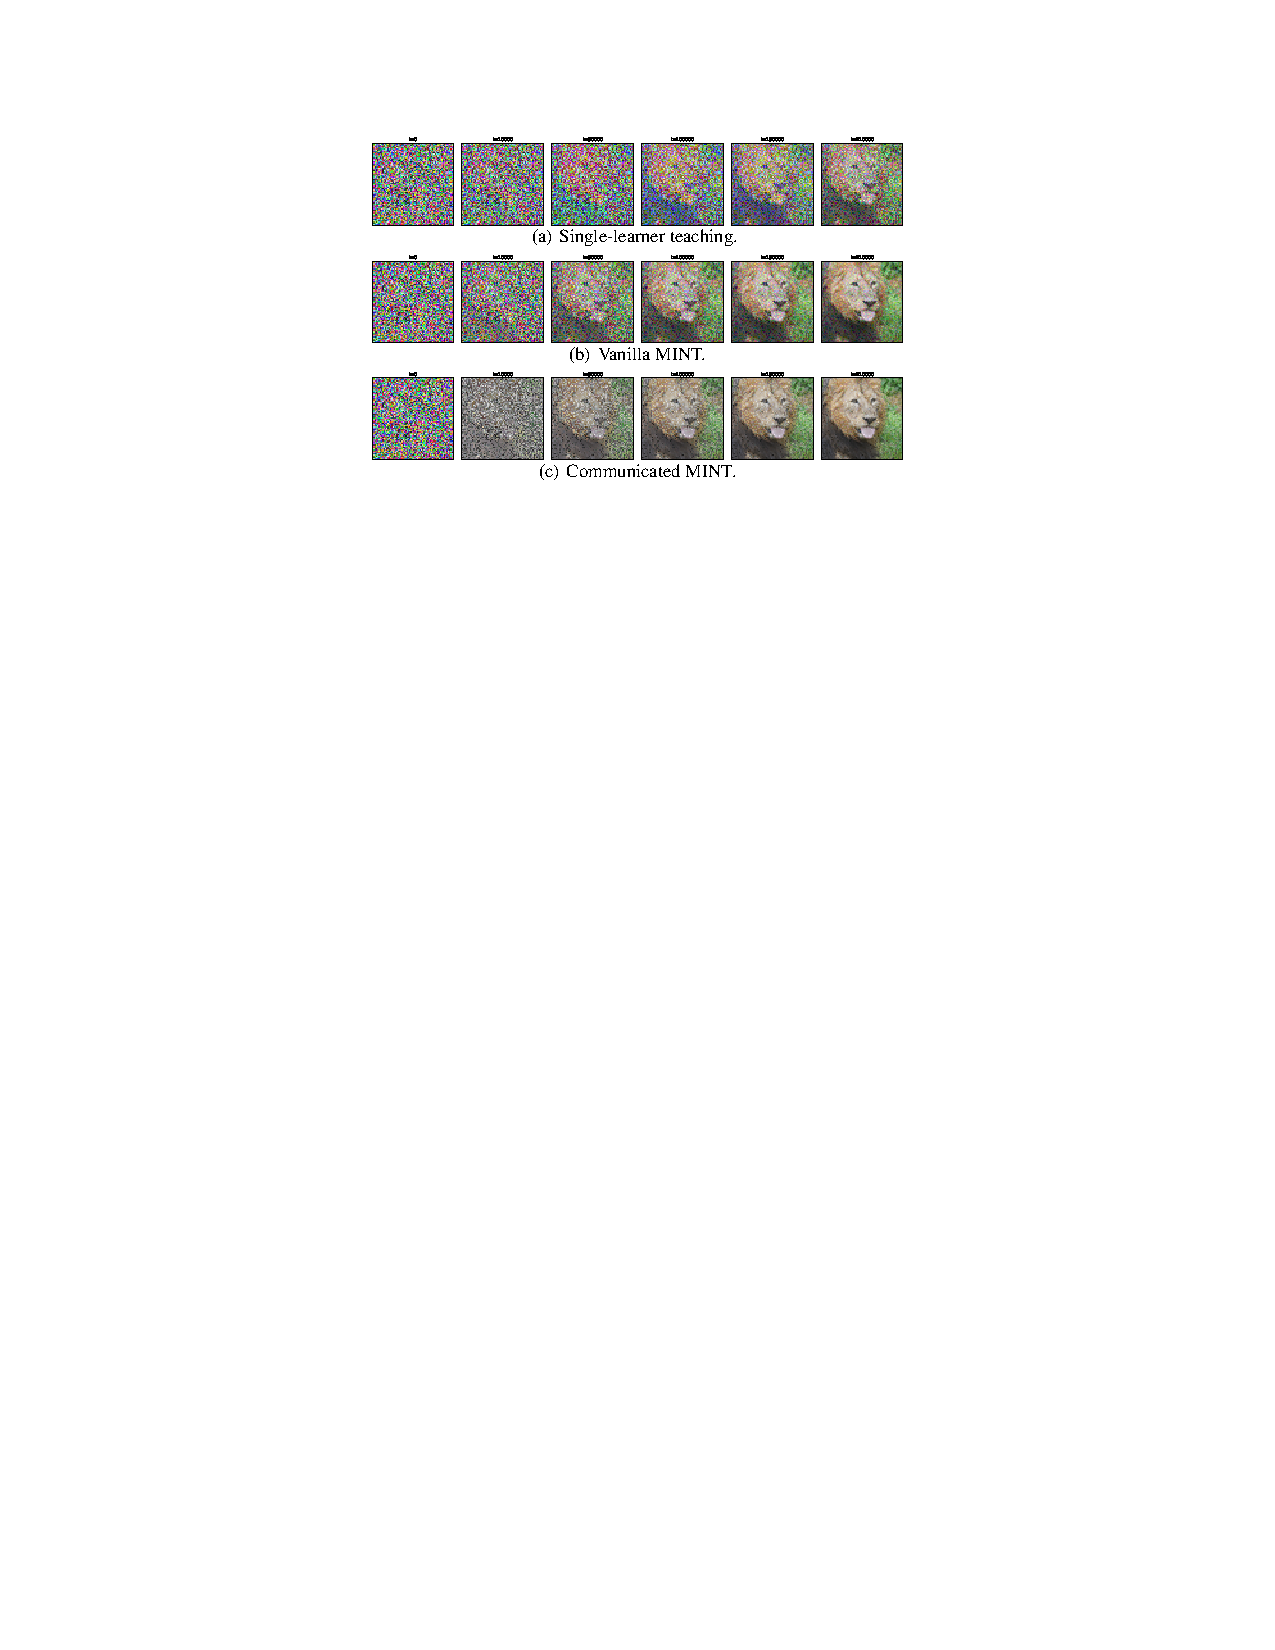
\includegraphics[width=\linewidth]{./out/RGBlion}

\end{block}

\end{column}

\end{columns}
\end{frame}

\end{document}

%%%%%%%%%%%%%%%%%%%%%%%%%%%%%%%%%%%%%%%%%%%%%%%%%%%%%%%%%%%%%%%%%%%%%%%%%%%%%%%%%%%%%%%%%%%%%%%%%%%%
%%% Local Variables: 
%%% mode: latex
%%% TeX-PDF-mode: t
%%% End: 